\documentclass[a4paper]{article}

%% Language and font encodings
\usepackage[english]{babel}
\usepackage[utf8x]{inputenc}
\usepackage[T1]{fontenc}
\usepackage{changepage}


%% Sets page size and margins
\usepackage[a4paper,top=3cm,bottom=2cm,left=3cm,right=3cm,marginparwidth=1.75cm]{geometry}

%% Useful packages
\usepackage{dsfont}
\usepackage{amsmath}
\usepackage{graphicx}
\usepackage[colorinlistoftodos]{todonotes}
\usepackage{indentfirst}
\usepackage[colorlinks=true, allcolors=blue]{hyperref}
\usepackage{setspace}
\usepackage{pgfplots}
\pgfplotsset{compat=1.14}

\title{MA108 Tutorial Solutions}
\author{Varun Patil}

\begin{document}
\maketitle 
\vspace{-8mm}
\begin{center}Disclaimer: This document was created Just for Fun!
\\I am not responsible for inaccuracies, bad solutions, burnt answer sheets or any thermonuclear war that this could cause. If you point your finger at me, I will just laugh at you.\end{center}

\section{Tutorial Sheet 1}
\renewcommand{\labelenumii}{(\roman{enumii})}

\doublespacing
\begin{enumerate}
\item{Classify the following equations (order, linear or non-linear):}
\begin{enumerate}
\item{\(\frac{d^3y}{dx^3} + 4(\frac{dy}{dx})^2=y\)
 \\Order : 3, non-linear
}
\item{\(\frac{dy}{dx}+2y=\sin x\)
 \\Order : 1, linear
}
\item{\(y\frac{d^2y}{dx^2}+2x\frac{dy}{dx}+y=0\)
 \\Order : 2, non-linear}
\item{\(\frac{d^4y}{dx^4}+(\sin x)\frac{dy}{dx}+x^2y=0\)
\\Order : 4, linear}
\item{\((1+y^2)\frac{d^2y}{dt^2}+t\frac{d^6y}{dt^6}+y=e^t\)
\\Order : 6, non-linear}
\end{enumerate}

\item{Formulate the differential equtions represented by the following functions by eliminating the arbitrary constants $a$, $b$ and $c$}:

\begin{enumerate}
\item{$y=ax^2$
\\$\frac{y}{x^2}=a$
\\Differentiating both sides wrt $x$,
\\$\frac{1}{x^2}\frac{dy}{dx} - \frac{2y}{x^3} = 0$
}
\item{$y-a^2=a(x-b)^2$
\\Differentiating both sides wrt $x$,
\\$\frac{dy}{dx}=2a(x-b)$
\\$\frac{1}{(x-b)}\frac{dy}{dx}=2a$
\\Differentiating both sides wrt $x$,
\\$\frac{1}{(x-b)}\frac{d^2y}{dx^2}-\frac{1}{(x-b)^2}\frac{dy}{dx}=0$
\\$\frac{d^2y}{dx^2}=\frac{dy}{dx}\frac{1}{(x-b)}$
\\$x-b=\frac{\frac{dy}{dx}}{\frac{d^2y}{dx^2}}$
\\$a=\frac{1}{2(x-b)}\frac{dy}{dx}=\frac{1}{2}\frac{d^2y}{dx^2}$
\\Substituting $a$ and $x-b$ in original equation,
\\$y - \frac{1}{4}(\frac{d^2y}{dx^2})^2=\frac{1}{2}\frac{d^2y}{dx^2}(\frac{\frac{d^2y}{dx^2}}{\frac{dy}{dx}})^2$
}

\item{$x^2+y^2=a^2$
\\Differentiating both sides wrt $x$,
\\$2x\frac{dy}{dx}+2y=0$
}

\item{$(x-a)^2+(y-b)^2=a^2$ \ ... (1)
\\Differentiating both sides wrt $x$,
\\$2(x-a)+2(y-b)\frac{dy}{dx}=0$ \ ... (2)
\\$\frac{(x-a)}{(y-b)} = -\frac{dy}{dx}$ \ ... (3)
\\Differentiating (2) wrt $x$,
\\$1+(y-b)\frac{d^2y}{dx^2}+(\frac{dy}{dx})^2=0$
\\$y-b=-\frac{1+(\frac{dy}{dx})^2}{\frac{d^2y}{dx^2}}$
\\Substituting $(y-b)$ in (2),
\\$a=x+(y-b)\frac{dy}{dx}$
\\$a=x-\frac{1+(\frac{dy}{dx})^2}{\frac{d^2y}{dx^2}}\frac{dy}{dx}$
\\Dividing (1) on both sides by $(y-b)^2$,
\\$\frac{(x-a)^2}{(y-b)^2} +1 = \frac{a^2}{(y-b)^2}$
\\$(\frac{dy}{dx})^2 +1=\frac{(x-\frac{1+(\frac{dy}{dx})^2}{\frac{d^2y}{dx^2}}\frac{dy}{dx})^2}{(\frac{1+(\frac{dy}{dx})^2}{\frac{d^2y}{dx^2}})^2}$
}

\item{$y=a\sin x + b \cos x +a$ ... (1)
\\Differentiating both sides wrt $x$,
\\$\frac{dy}{dx}=a\cos x - b\sin x$ ... (2)
\\Multiply (1) by $\sin x$ and (2) by $\cos x$ and add,
\\$y\sin x+\frac{dy}{dx}\cos x = a\sin ^2 x + a \cos ^2 x +a\sin x$
\\$y\sin x+\frac{dy}{dx}\cos x = a(1+\sin x)$
\\$a=\frac{y\sin x+\frac{dy}{dx}\cos x}{1+\sin x}$ ...(3)
\\Differentiating both sides of (2) wrt $x$
\\$\frac{d^2y}{dx^2}=-(a\sin x + b\cos x)$ ... (4)
\\Adding (1) and (4),
\\$y+\frac{d^2y}{dx^2}=a$
\\From equation (4),
\\$y+\frac{d^2y}{dx^2}=\frac{y\sin x+\frac{dy}{dx}\cos x}{1+\sin x}$
}

\item{$y=a(1-x^2)+bx +cx^3$
\\Differentiating both sides wrt $x$
\\$\frac{dy}{dx}=-2ax+b+3cx^2$ ...(1)
\\Differentiating both sides wrt $x$
\\$\frac{d^2y}{dx^2}=-2a+6cx$ ... (2)
\\Differentiating both sides wrt $x$
\\$\frac{d^3y}{dx^3}=6c$ ...(3)
\\From (2) and (3),
\\$\frac{d^2y}{dx^2}=-2a+x\frac{d^3y}{dx^3}$ ...(4)
\\From (3), (4) and (1),
\\$\frac{dy}{dx}=x(\frac{d^2y}{dx^2}-x\frac{d^3y}{dx^3})+b+\frac{x^2}{2}\frac{d^3y}{dx^3}$
\\From all equations,
\\$y=-\frac{1}{2}(\frac{d^2y}{dx^2}-x\frac{d^3y}{dx^3})(1-x^2)+(\frac{dy}{dx}-x(\frac{d^2y}{dx^2}-x\frac{d^3y}{dx^3})-\frac{x^2}{2}\frac{d^3y}{dx^3})x+ (\frac{1}{6}\frac{d^3y}{dx^3}) x^3$
}

\item{$y=cx+f(c)$
\\Differentiating both sides wrt $x$
\\$\frac{dy}{dx}=c$
\\$y=\frac{dy}{dx}+f(\frac{dy}{dx})$

}
\end{enumerate}

\item{Solve the equation $x^3(\sin y)y' = 2$. Find the particular solution such that $y(x) \rightarrow  \frac{\pi}{2}$ as $x \rightarrow +\infty$.
\\$x^3(\sin y)\frac{dy}{dx}=2$
\\$(\sin y)dy=\frac{2}{x^3}dx$
\\$\int(\sin y)dy=\int\frac{2}{x^2}dx$
\\$-\cos y+c=-\frac{2}{x}$
\\$\frac{2}{x}-\cos y+c=0$
\\This is an implicit solution for the given differential equation.
\\As $x\rightarrow\infty$, $\frac{2}{x}\rightarrow 0$ and as $y(x) \rightarrow  \frac{\pi}{2}$, $\cos y\rightarrow 0$
\\$\implies c=0$
\\$\frac{2}{x}-\cos y=0$ is the required particular solution.
}

\item{Prove that a curve with the property that all its normals pass through a point is a circle.
\\Let $(x_0, y_0)$ be a point on the curve
\\Equation of normal at $(x_0, y_0)$ is $-\frac{x_0-x}{y_0-y}=\frac{dy}{dx}$
\\Let the point $(a, b)$ always satisfy this equation, i.e. $(x_0, y_0) \equiv (x, y)$
\\$\implies -\frac{x-a}{y-b}=\frac{dy}{dx}$
\\$\implies -(x-a)dx = (y-b)dy$
\\$\implies \int -(x-a)dx = \int (y-b)dy$
\\$\implies -(x-a)^2 + c = (y-b)^2 $
\\$\implies (x-a)^2 + (y-b)^2 =c $
\\This is a real curve iff $c=r^2$, where $r$ is a real number.
\\Therefore, it is the equation of a circle with center at $(a, b)$.
}
\renewcommand{\labelenumii}{(\alph{enumii})}
\item{Find the values of m for which
\begin{enumerate}
\item{$y=e^{mx}$ is a solution of
\begin{enumerate}
\item{$y'' +y'-6y=0$
\\Substituting $y=e^{mx}$ in the given equation,
\\$m^2e^{mx}+me^{mx}-6e^{mx}=0$
\\$m^2+m-6=0$
\\$(m+3)(m-2)=0$
\\$\implies m=-3$ or $m=2$
}
\item{$y'''-3y''+2y'=0$
\\Substituting $y=e^{mx}$ in the given equation,
\\$m^3e^{mx}-3m^2e^{mx}+2me^{mx}=0$
\\$m^3-3m^2+2m=0$
\\$m(m-2)(m-1)=0$
\\$\implies m=0$ or $m=2$ or $m=1$
}

\end{enumerate}
}

\item{$y=x^m$ for $x>0$ is a solution of}
\begin{enumerate}
\item{$x^2y''-4xy'+4y=0$
\\Substituting $y=x^m$ in the given equation,
\\$x^2m(m-1)x^{m-2}-4xmx^{m-1}+4x^m=0$
\\Dividing by $x^m$,
\\$m(m-1)-4m+4=0$
\\$\implies m=4$ or $m=1$
}
\item{$x^2y'''-xy''+y'=0$
\\Substituting $y=x^m$ in the given equation,
\\$x^2m(m-1)(m-2)x^{m-3}-xm(m-1)x^{m-2}+mx^{m-1}=0$
\\Dividing by $x^{m-1}$,
\\$m(m-1)(m-2)-m(m-1)+m=0$
\\$m(m^2-3m+2-m^2+m+m)=0$
\\$m(2-m)=0$
\\$\implies m=0$ or $m=2$
}
\end{enumerate}
\end{enumerate}
}
\renewcommand{\labelenumii}{(\roman{enumii})}
\item{For each of the following linear differential equations verify that the function given in brackets is a solution of the differential equation.
\\ \textbf{Warning : Incomplete.}
\begin{enumerate}
\item{$y''+4y=5e^x+3\sin x \ (y=a\sin 2x+ b\cos 2x+e^x+\sin x)$
\item{$y''-5y'+6y=0 \ (y_1=e^{3x}, y_2=e^{2x}, c_1y_1+c_2y_2)$}
\item{$y'''+6y''+11y'+6y=e^{-2x} \ (y=ae^{-x}+be^{-2x}+ce^{-3x}-xe^{-2x})$}
\item{$y''' +8y=9e^x=65\cos x \ (y=ae^{-2x}+e^x(b\cos \sqrt[]{3}x+c\sin \sqrt[]{3}x)+8\cos x-\sin x	+e^x)$}


}


\end{enumerate}

\item{Let $\phi_i$ be a solution of $y' +ay=b_i(x)$ for $i$=1,2. Show that $\phi_1+\phi_2$ satisfies $y' +ay=b_1(x)+b_2(x)$. Use this result to find the solutions of $y'+y=\sin x+ 3\cos 2x$ passing through the origin.
\\The proof follows immediately from the fact that the equation is linear and hence,
\\$(\phi_1+\phi_2)'+a(\phi_1+\phi_2)=(\phi_1)'+(\phi_2)' + a\phi_1+a\phi_2$
\\$=(\phi_1'+ a\phi_1) +(\phi_2' +a\phi_2)$
\\$=b_1(x)+b_2(x)$
\\Let $b_1=\sin x$ and $b_2=3\cos 2x$
\\For $\phi_1$, we have,
\\$\phi_1' + a\phi_1=\sin x$
\\Multiplying both sides by $e^{ax}$,
\\$e^{ax}\phi_1' + ae^{ax}\phi_1=e^{ax}\sin x$
\\$(\phi_1e^{ax})'=e^{ax}\sin x$
\\$\phi_1e^{ax}=\int e^{ax}\sin x \ dx=e^{ax}\frac{(a\sin x - \cos x)}{a^2+1} +c$
\\$\phi_1=\frac{a\sin x - \cos x}{a^2+1} +c$
\\Similarly,
\\$\phi_2=\frac{3(a\cos 2x+2\sin 2x)}{a^2+4}$
\\The required solutions are $\phi_1+\phi_2$
}
}
\item{Obtain the solution of the following differential equations:
\begin{enumerate}
\item{$(x^2+1)dy+(y^2+4)dx=0$; $y(1)=0$
\\$\frac{dy}{y^2+4}=-\frac{dx}{x^2+1}$
\\$\int\frac{dy}{y^2+4}=-\int\frac{dx}{x^2+1}$
\\$\frac{1}{2}\tan^{-1}{\frac{y}{2}}=-\tan^{-1}{x}+c$
\\$\frac{1}{2}\tan^{-1}{\frac{y}{2}}+\tan^{-1}{x}=c$
\\Putting $x=1$, $y=0$,
\\$c=\frac{\pi}{4}$ is the constant for the particular solution.
}
\item{$y'=y\cot x$; $y(\frac{\pi}{2})=1$
\\$\frac{dy}{dx}=\frac{y}{\tan x}$
\\$\frac{dy}{y}=\frac{\cos x}{\sin x}dx$
\\$\int\frac{dy}{y}=\int\frac{\cos x}{\sin x}dx$
\\$\ln{y}=\ln{\sin x} +c$
\\$y=c\sin x$
\\Putting $x=\frac{\pi}{2}$, $y=1$,
\\$c=1$ is the constant for the particular solution.
}
\item{$y'=y(y^2-1)$, with $y(0)=2$ or $y(0)=1$ or $y(0)=0$
\\$\frac{dy}{dx}=y(y^2-1)$
\\$\int\frac{dy}{y(y-1)(y+1)}=\int dx$
\\Using partial fractions,
\\$\int(\frac{A}{y}+\frac{B}{y-1}+\frac{C}{y+1})dy=\int dx$
\\$A=-1, B=C=\frac{1}{2}$
\\$\implies -\ln{y} + \frac{1}{2}\ln{|y-1|} + \frac{1}{2}\ln{|y+1|}=x+c$
\\On putting values for $(x, y)$ as $(0, 2), (0, 1)$ and $(0, 0)$, we get the respective particular solutions.
}
\item{$(x+2)y'-xy=0$; $y(0)=1$
\\$(x+2)\frac{dy}{dx}=xy$
\\$\frac{dy}{y}=\frac{x}{x+2}dx$
\\$\int\frac{dy}{y}=\int(\frac{x}{x+2})dx$
\\$\int\frac{dy}{y}=\int(1 - \frac{2}{x+2})dx$
\\$\ln y = x - 2\ln|x+2| + c$
\\Putting $x=0$, $y=1$,
\\$0=-2\ln 2 +c$
\\$c=\ln 4$ is the constant for the particular solution.
}
\item{$y'+\frac{y-x}{y+x}=0$; $y(1)=1$
\\Substituting $y=vx$, $y'=v'x + v$,
\\$v'x+v+\frac{vx-x}{vx+x}=0$
\\$v'x+v+\frac{v-1}{v+1}=0$
\\$\frac{dv}{dx}x =\frac{1-v}{1+v}-v$
\\$\frac{dv}{dx}x =\frac{1-2v-v^2}{1+v}$
\\$\frac{1+v}{1-2v-v^2}dv=\frac{1}{x}dx$
\\$\int\frac{1+v}{1-2v-v^2}dv=\int\frac{1}{x}dx$
\\$-\frac{1}{2}\ln|1-2v-v^2|=\ln x +c$
\\$\frac{1}{\sqrt[]{|1-2v-v^2|}}=cx$
\\$\frac{x}{\sqrt[]{|x^2-2xy-y^2|}}=cx$
\\$\frac{}{\sqrt[]{|x^2-2xy-y^2|}}=c$
\\Putting $x=1$, $y=1$,
\\$c=\frac{1}{\sqrt[]{2}}$ is the constant for the particular solution.
}
\item{$y'=(y-x)^2$; $y(0)=2$
\\Substituting $v=y-x$, $v'=y'-1$,
\\$v'+1=v^2$
\\$\int \frac{dv}{v^2-1}=\int dx$
\\$\frac{1}{2}\ln(\frac{v-1}{v+1})=x+c$
\\$\ln(c_1\frac{v-1}{v+1})=2x$
\\$\frac{v-1}{v+1}=c_2e^{2x}$
\\$\frac{y-x-1}{y-x+1}=c_2e^{2x}$
\\Putting $x=0$, $y=2$,
\\$\frac{1}{3}=c_2$ is the constant for the particular solution.
}
\item{$2(y\sin 2x+\cos 2x)dx=\cos 2x \ dy$; $y(\pi)=0$
\\Substituting $v=y\cos 2x$, $dv=dy\cos 2x - 2y\sin 2x \ dx$,
\\$2(y\sin 2x+\cos 2x)dx=dv+2y\sin 2x \ dx$
\\$\int 2\cos 2x \ dx=\int dv$
\\$\sin 2x = v+c$
\\$\sin 2x = y\cos 2x + c$
\\Putting $x=\pi$, $y=0$,
\\$c=0$ is the constant for the particular solution.
}
\item{$y'=\frac{1}{(x+1)(x^2+1)}$
\\$\frac{dy}{dx}=\frac{1}{(x+1)(x^2+1)}$
\\$\int dy=\int\frac{dx}{(x+1)(x^2+1)}$
\\Putting $x=\tan \theta$,
\\$y=\int \frac{\sec ^2 \theta}{(\tan \theta +1)(\tan ^2 \theta +1)} d\theta$
\\$y=\int \frac{\cos \theta}{\sin \theta + \cos \theta} d\theta$
\\$y=\int \frac{1}{2} (\frac{\cos \theta + \sin \theta}{\cos \theta + \sin \theta} + \frac{\cos \theta - \sin \theta}{\cos \theta + \sin \theta})d\theta$
\\$y=\int \frac{1}{2} (1 + \frac{\cos \theta - \sin \theta}{\cos \theta + \sin \theta})d\theta$
\\$y=\frac{1}{2}(\theta + \ln|\cos \theta + \sin \theta|) +c$
\\$y=\frac{1}{2}(\tan^{-1}x + \ln|\frac{1+x}{\sqrt[]{1+x^2}}|)+c$
\\This is the general solution for the differential equation.
}
\end{enumerate}

}

\item{For each of the following differential equations, find the general solution (by substituting $y = vx$)
\begin{enumerate}
\item{$y'=\frac{y^2-xy}{x^2+xy}$
\\Substituting $y=vx$, $y'=v'x+v$,
\\$v'x+v=v\frac{v-1}{v+1}$
\\$x\frac{dv}{dx}=v(\frac{v-1}{v+1}-1)$
\\$x\frac{dv}{dx}=-\frac{2}{v+1}$
\\$\int (v+1) dv=\int \frac{-2}{x}dx$
\\$\frac{v^2}{2}+v=-2\ln |x| +c$
\\$\frac{v^2}{2}+v=\ln c_1x^{-2}$
\\$\frac{1}{2}(\frac{y}{x})^2+\frac{y}{x}=\ln c_1x^{-2}$ is the general solution for the given differential equation.
}
\item{$x^2y'=y^2+xy+x^2$
\\Substituting $y=vx$, $y'=v'x+v$,
\\$x^2(v'x+v)=v^2x^2+vx^2+x^2$
\\$v'x+v=v^2+v+1$
\\$v'x=v^2+1$
\\$\frac{dv}{v^2+1}=dx$
\\$\int \frac{dv}{v^2+1}=\int dx$
\\$\tan^{-1}v=x+c$
\\$\tan^{-1}\frac{y}{x}=x+c$ is the general solution for the given differential equation.
}
\item{$xy'=y+x\cos^2(\frac{y}{x})$
\\Substituting $y=vx$, $y'=v'x+v$,
\\$x(v'x+v)=vx+x\cos^2v$
\\$v'x=\cos^2v$
\\$\int \frac{dv}{\cos^2v}=\int\frac{dx}{x}$
\\$\tan v=\ln |x|+c$ 
\\$e^{\tan \frac{y}{x}} = c_1|x|$ is the general solution for the given differential equation.
}
\item{$xy'=y(\ln y-\ln x)$
\\Substituting $y=vx$, $y'=v'x+v$,
\\$x(v'x+v)=vx\ln v$
\\$v'x=v(\ln v -1)$
\\$\int \frac{dv}{v(\ln v -1)}=\int\frac{dx}{x}$
\\$\ln|\ln v - 1| = \ln |x| + c$
\\$\ln v - 1 = c_1x$ is the general solution for the given differential equation.
}

\end{enumerate}
}

\item{Show that the differential equation $\frac{dy}{dx}=\frac{ax+by+m}{cx+dy+n}$ where $a, b, c, d, m$ and $n$ are constants can be reduced to $\frac{dy}{dt}=\frac{ax+by}{cx+dy}$ if $ad-bc\neq 0$. Then find the general solution of the given equations.
\\ \textbf{Warning : Incomplete.}
\begin{enumerate}
\item{$(1+x-2y)+y'(4x-3y-6)=0$}
\item{$y'=\frac{y-x+1}{y-x+5}$}
\item{$(x+2y+3)+(2x+4y-1)y'=0$}
\end{enumerate}
}

\item{Solve the differential equation $\sqrt[]{1-y^2} \ dx + \sqrt{1-x^2} \ dy=0$ with the conditions $y(0)=\frac{\pm1}{2}\sqrt[]{3}$. Sketch the graphs of the solutions and show that they are each arcs of the same ellipse. Also show that after these arcs are removed, the remaining part of the ellipse does not satisfy the differential equation.
\\$\sqrt[]{1-y^2} \ dx + \sqrt{1-x^2} \ dy=0$
\\Dividing by $\sqrt[]{1-y^2}\sqrt{1-x^2}$
\\$\frac{dx}{\sqrt[]{1-x^2}}+\frac{dy}{\sqrt[]{q-y^2}}=0$
\\$\int\frac{dx}{\sqrt[]{1-x^2}}+\int\frac{dy}{\sqrt[]{1-y^2}}=0$
\\$\sin^{-1}x+\sin^{-1}y=c$
\\Putting $x=0$ and $y=\frac{\sqrt[]{3}}{2}$,
\\$c_1=\frac{\pi}{3}$
\\Putting $x=0$ and $y=-\frac{\sqrt[]{3}}{2}$,
\\$c_2=-\frac{\pi}{3}$
\\(Where $c_1$ and $c_2$ are the constants for the two particular solutions)
\\Since $\frac{dy}{dx}<0$, we need to exclude the regions of the solution where $\frac{dy}{dx}>0$
\\
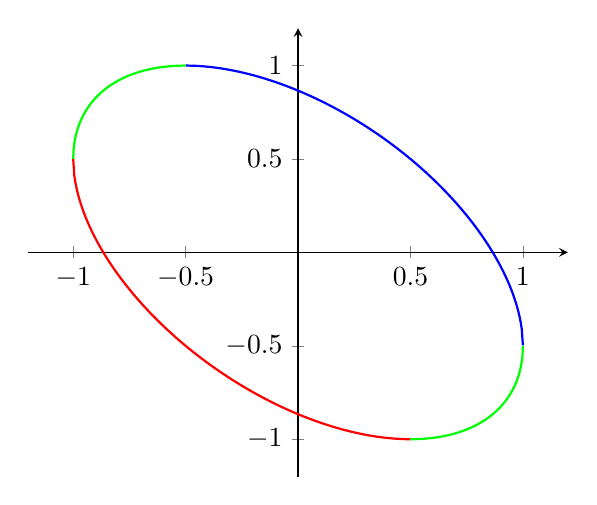
\begin{tikzpicture}
\begin{axis}[
    trig format plots=rad,
    samples=300,
    axis lines=middle, enlargelimits=true
]
\addplot [no markers,blue,thick,domain=-1/2:1
] {sin((pi/3)-asin(x))};

\addplot [no markers,green,thick,domain=-1:-1/2
] {sin((pi/3)-asin(x))};

\addplot [no markers,red,thick,domain=-1:1/2
] {sin((-pi/3)-asin(x))};

\addplot [no markers,green,thick,domain=1/2:1
] {sin((-pi/3)-asin(x))};

\end{axis}
\end{tikzpicture}
\\
\\The blue part of the graph corresponds to $c=\frac{\pi}{3}$ and the red part corresponds to $c=-\frac{\pi}{3}$. The green part of the ellipse is not a solution to the differential equation.
}

\item{The differential equation $y=xy'+f(y')$ is called a Clairaut equation (or Clairaut's equation). Show that the general solution of this equation is the family of straight lines $y=cx + f(c)$. In addition to these, show that it has a special solution given by $f'(p)=-x$ where $p=y'$. This special solution which does not (in general) represent one of the straight lines $y=cx+f(c)$, is called a singular solution. Hint: Differentiate the differential equation.
\\$y=xy'+f(y')$
\\Differentiation both sides wrt $x$,
\\$y'=y'+xy''+f(y')y''$
\\$y''(x+f(y'))=0$
\\$\implies y''=0$ or $x+f(y')=0$
\\$\implies y'=c$ or $f'(p)=-x$, where $p=y'$
\\Substituting $y'=c$ in Clairaut's equation,
\\$y=cx+f(c)$ is the general solution
\\$f'(p)=-x$, where $p=y'$ is the singular solution
}

\item{Determine the general solutions as well as the singular solutions of the following Clairaut equations.\textit{ In each of the two examples, sketch the graphs of these solutions.}
\\ \textbf{Warning : Incomplete.}
\begin{enumerate}
\item{$y=xy'+\frac{1}{y'}$
\\Since the equation is in the form of a Clairaut equation with $f(x)=\frac{1}{x}$, we can substitute $y'=c$ to get the general solution.
\\$y=cx+\frac{1}{c}$ is the general solution of the differential equation.
\\Let $p=y'$ and $f'(p)=-x$,
\\$-\frac{1}{p^2}=-x$
\\$p=\frac{1}{\sqrt[]{x}}$
\\Substitute $y'=p=\frac{1}{\sqrt[]{x}}$ in the equation,
\\$y=\frac{x}{\sqrt[]{x}}+\sqrt[]{x}$
\\$\implies y=2 \ \sqrt[]{x}$ is the singular solution of the equation.
}
\item{$y=xy'-\frac{y'}{\sqrt[]{1+y'^2}}$
\\Since the equation is in the form of a Clairaut equation with $f(x)=-\frac{x}{\sqrt[]{1+x^2}}$, we can substitute $y'=c$ to get the general solution.
\\$y=cx-\frac{c}{\sqrt[]{1+c^2}}$ is the general solution of the differential equation.
\\Let $p=y'$ and $f'(p)=-x$,
\\$\frac{d}{dp}(\frac{p}{\sqrt[]{1+p^2}})=-x$
\\$\frac{1}{(1+p^2)^{3/2}}=-x$
\\$p=\sqrt[]{\frac{1}{x^{2/3}}-1}$
\\Substitute $y'=p=\sqrt[]{\frac{1}{x^{2/3}}-1}$ in the equation,
\\$y=x\sqrt[]{\frac{1}{x^{2/3}}-1}-\sqrt[]{1-x^{2/3}}$
\\$y=-(1-x^{2/3})^{3/2}$ is the singular solution of the equation.
}
\end{enumerate}
}
\item{For the parabola $y=x^2$ find the equation of its tangent at $(c, c^2)$ and find the ordinary differential equation for this one parameter family of tangents. Identify this as a Clairaut equation. More generally, take your favorite curve and determine the ODE for the one parameter family of its tangents and verify that it is a Clairaut's equation. N.B: Exercise 13 shows that the converse is true.
\\$\frac{dy}{dx}=2x$
\\Equation of tangent at $(c, c^2)$ is,
\\$\frac{y-c^2}{x-c}=2c$
\\$y=2cx-c^2$
\\Put $c_1=2c$
\\$y=c_1x-(\frac{c_1}{2})^2$
\\This is a solution for the Clairaut equation:
\\$y=xy'-(\frac{y'}{2})^2$
\\Similarly for other curves, the one parameter family of tangents forms a Clairaut equation.
}

\item{In the preceding exercises, show that in each case, the envelope of the family of straight lines is also a solution of the Clairaut equation.
\\For the envelope of the family of lines, we have,
\\$F(x,y,c)=y-2cx+c^2=0$
\\$\frac{\partial F(x,y,c)}{\partial c}=-2x+2c=0$
\\$\implies x=c, y=c^2 \implies y=x^2$, i.e. the equation of the parabola itself.
\\Substituting $y=x^2$ in the equation
\\$y=xy'-(\frac{y'}{2})^2$
\\$x^2=2x^2-(\frac{2x}{2})^2 \implies 1=1$ 
\\Thus, the envelope of the family of lines satisfies the Clairaut equation.
\\Similar for other curves.
}

\item{Show that the differential equation $y'-y^3=2x^{-3/2}$ has three distinct solutions of the form $\frac{A}{\sqrt[]{x}}$ but that only one of these is real valued.
\\Putting $y=\frac{A}{\sqrt[]{x}}$ in the given equation,
\\$-\frac{1}{2}\frac{A}{x^{3/2}}-\frac{A^3}{x^{3/2}}=\frac{2}{x^{3/2}}$
\\$\frac{2}{x^{3/2}}+\frac{1}{2}\frac{A}{x^{3/2}}+\frac{A^3}{x^{3/2}}=0$
\\$\implies Q=2A^3+A+4=0$
\\$\implies A$ can have only one real value, since $Q \rightarrow \infty$ as $A \rightarrow \infty$; $Q \rightarrow -\infty$ as $A \rightarrow -\infty$ and $\frac{dQ}{dA}>0$, i.e. Q is always increasing.
}
\end{enumerate}

\section{Tutorial Sheet 2}
\begin{enumerate}
\item{State the conditions under which the following equations are exact.
\textbf{\\Warning: This solution is suspicious!}
\begin{enumerate}
\item{$[f(x)+g(y)]dx+[h(x)+k(y)]dy=0$
\\For the equation to be exact on ${\rm I\!R^2}$, it must be closed,
\\$\implies \frac{\partial f(x)+g(y)}{\partial y} = \frac{\partial h(x)+k(y)}{\partial x}$
\\$\implies g'(y)=h'(x)$
\\For this to be true always, both must be equal to zero.
\\$\implies g'(y)=h'(x)=c$
\\$\implies g(y)=cy, h(x)=cx$
}

\item{$(x^3+xy^2)dx+(ax^2y+bxy^2)dy=0$
\\For the equation to be exact on ${\rm I\!R^2}$, it must be closed,
\\$\implies \frac{\partial (x^3+xy^2)}{\partial y}=\frac{\partial (ax^2y+bxy^2)}{\partial x}$
\\$\implies 2xy=2axy+by^2$
\\$\implies 2x=2ax+by$
\\$\implies a=1, b=0$
}

\item{$(ax^2+2bxy+cy^2)dx + (bx^2+2cxy+gy^2)dy=0$
\\For the equation to be exact on ${\rm I\!R^2}$, it must be closed,
\\$\implies \frac{\partial (ax^2+2bxy+cy^2)}{\partial y}=\frac{\partial (bx^2+2cxy+gy^2)}{\partial x}$
\\$\implies 2bx+2cy=2cy+2bx$
\\$\implies$ The equation is always exact.
}

\end{enumerate}
}

\item{Solve the following exact equations
\begin{enumerate}
\item{$3x(xy-2)+(x^3+2y)dy=0$
\\Let $M(x,y)=3x(xy-2)$ and $N(x,y)=(x^3+2y)$
\\Let $u(x,y)$ be a function such that $\frac{\partial u(x,y)}{\partial x}=M(x,y)$ and $\frac{\partial u(x,y)}{\partial y}=N(x,y)$
\\$\implies u=\int 3x(xy-2) \ dx +c(y)$
\\$\implies u=\int 3x^2y - 6x \ dx +c(y)$
\\$\implies u=x^3y - 3x^2 +c(y)$
\\Partially differentiating $u(x,y)$ wrt $y$,
\\$\frac{\partial u(x,y)}{\partial y}=N(x,y)$
\\$\implies \frac{\partial (x^3y - 3x^2 +c(y))}{\partial y}=x^3+2y$
\\$\implies x^3+c'(y)=x^3+2y$
\\$\implies c'(y)=2y$
\\$\implies c(y)=y^2+c_1$
\\$\implies$ The solution to the differential equation is $x^3y - 3x^2 +y^2=c_2$
}

\item{$(\cos x \cos y - \cot x) dx - \sin x \sin y \ dy =0$
\\Let $M(x,y)=\cos x \cos y - \cot x$ and $N(x,y)=\sin x \sin y$
\\Let $u(x,y)$ be a function such that $\frac{\partial u(x,y)}{\partial x}=M(x,y)$ and $\frac{\partial u(x,y)}{\partial y}=N(x,y)$
\\$\implies u=\int \cos x \cos y - \cot x \ dx + c(y)$
\\$\implies u=\sin x \cos y - \ln\sin x + c(y)$
\\Partially differentiating $u(x,y)$ wrt $y$,
\\$\frac{\partial u(x,y)}{\partial y}=N(x,y)$
\\$\implies\frac{\partial (\sin x \cos y - \ln\sin x + c(y))}{\partial y}=\sin x \sin y$
\\$\implies -\sin x \sin y+c'(y)=\sin x \sin y$
\\$\implies c'(y)=2\sin x \sin y$
\\$\implies c(y)=-2\sin x \cos y+c_1$
\\$\implies$ The solution to the differential equation is $\sin x \cos y - \ln\sin x -2\sin x \cos y=c_2$
}

\item{$e^xy(x+y)dx+e^x(x+2y-1)dy=0$
\\Let $M(x,y)=e^xy(x+y) - \cot x$ and $N(x,y)=e^x(x+2y-1)$
\\Let $u(x,y)$ be a function such that $\frac{\partial u(x,y)}{\partial x}=M(x,y)$ and $\frac{\partial u(x,y)}{\partial y}=N(x,y)$
\\$\implies u=\int e^x y(x+y) \ dx +c(y)$
\\$\implies u=\int e^x xy + e^x y^2 \ dx +c(y)$
\\$\implies u=y\int xe^x \ dx + e^x y^2 +c(y)$
\\$\implies u=e^x y(x-1) + e^x y^2 +c(y)$
\\$\implies u=ye^x (x+y-1) +c(y)$
\\Partially differentiating $u(x,y)$ wrt $y$,
\\$\frac{\partial u(x,y)}{\partial y}=N(x,y)$
\\$\implies \frac{\partial (ye^x (x+y-1) +c(y))}{\partial y}=e^x(x+2y-1)$
\\$\implies \frac{\partial (ye^x (x-1) +y^2e^x +c(y))}{\partial y}=e^x(x+2y-1)$
\\$\implies e^x(x-1)+2ye^x +c'(y)= e^x(x+2y-1)$
\\$\implies c'(y)=0$
\\$\implies c(y)=c_1$
\\$\implies$ The solution to the differential equation is $ye^x (x+y-1)=c_2$
}
\end{enumerate}
}
\item{Determine (by inspection suitable) Integrating Factors (IF's) so that the following equations are exact. \\ \textbf{Warning : Incomplete.}
\begin{enumerate}
\item{$ydx+xdy=0$
\\The equation is exact, since $M_y=N_x$, hence an integrating factor is $1$.
}
\item{$d(e^x\sin y)=0$
\\The equation is exact, with solution $e^x\sin y=c$
}
\item{$dx+(\frac{y}{x})^2dy=0$
\\By inspection, multiplying both sides by the integrating factor $x^2$,
\\$x^2dx+y^2dy=0$
\\The equation is exact, since $M_y=N_x$
}
\item{$ye^{x/y}dx+(y-xe^{x/y}dy=0$
\\ \textbf{Warning : Incomplete.}
}
\item{$(2x+e^y)dx+xe^ydy=0$
\\The equation is exact, since $M_y=N_x$, hence an integrating factor is $1$.
}
\item{$(x^2+y^2)dx+xydy=0$
\\Trying the integrating factor $\frac{1}{x(x^2+2y^2)}$,
\\$(\frac{x^2+y^2}{x(x^2+2y^2)})dx+\frac{xy}{x(x^2+2y^2)}dy=0$
\\$(\frac{x^2+2y^2}{x(x^2+2y^2)}-\frac{y^2}{x(x^2+2y^2)})dx+\frac{y}{x^2+2y^2}dy=0$
\\$(\frac{1}{x}-\frac{y^2}{x(x^2+2y^2)})dx+\frac{y}{x^2+2y^2}dy=0$
\\$M_y=0-\frac{1}{x}\frac{2y(x^2+2y^2)-y^2(4y)}{(x^2+2y^2)^2}$
\\$M_y=-\frac{2xy}{(x^2+2y^2)^2}$
\\$N_x=-\frac{2xy}{(x^2+2y^2)^2}$
\\$\implies M_y=N_x$
\\Hence, $\frac{1}{x(x^2+2y^2)}$ is an integrating factor for the equation.
}
\end{enumerate}
}
\item{Verify that the equation $Mdx+Ndy=0$ ... (1) can be expressed in the form \[\frac{1}{2}(Mx+Ny)d(\ln xy) + \frac{1}{2}(Mx-Ny)d\ln(\frac{x}{y})=0\]
\\Expanding the differentials in the second equation,
\\$\frac{1}{2}(Mx+Ny)d(\ln xy) + \frac{1}{2}(Mx-Ny)d\ln(\frac{x}{y})=0$
\\$\frac{1}{2}(Mx+Ny)d(\ln x+ \ln y) + \frac{1}{2}(Mx-Ny)d(\ln x -\ln y)=0$
\\$\frac{1}{2}(Mx+Ny)(\frac{dx}{x}+ \frac{dy}{y}) + \frac{1}{2}(Mx-Ny)(\frac{dx}{x}- \frac{dy}{y})=0$
\\$Mdx+Ndy=0$
\\Hence, the equation can be expressed in the given form.
\\Hence, show that,
\begin{enumerate}
\item{if $Mx+Ny=0$, then $\frac{1}{Mx-Ny}$ is an IF of (1)
\\Multiplying the second equation by $\frac{1}{Mx-Ny}$, putting $Mx+Ny=0$,
\\$\frac{1}{2}(\frac{dx}{x} - \frac{dy}{y})=0$
\\This equation is exact, since $M_y=N_x$, hence $\frac{1}{Mx-Ny}$ is an integrating factor.
}

\item{if $Mx-Ny=0$, then $\frac{1}{Mx+Ny}$ is an IF of (1)
\\Multiplying the second equation by $\frac{1}{Mx+Ny}$, putting $Mx-Ny=0$,
\\$\frac{1}{2}(\frac{dx}{x} + \frac{dy}{y})=0$
\\This equation is exact, since $M_y=N_x$, hence $\frac{1}{Mx+Ny}$ is an integrating factor.
}

\item{if $M$ and $N$ are homogeneous of the same degree then $\frac{1}{Mx+Ny}$ is an IF of (1).
\\Multiplying the second equation by $\frac{1}{Mx+Ny}$,
\\$d(\ln xy) + \frac{(Mx-Ny)}{(Mx+Ny)}d\ln(\frac{x}{y})=0$
\\$d(\ln xy) + \frac{(1-\frac{Ny}{Mx})}{(1+\frac{Ny}{Mx})}d\ln(\frac{x}{y})=0$
\\Since $Ny$ and $Mx$ are homogeneous of the same degree, we can express $\frac{Ny}{Mx}$ purely as a function of $v$, where $v=\frac{y}{x}$
\\$d(\ln xy) + f(v)d\ln(\frac{x}{y})=0$
\\$d(\ln xy) + f(v)d\ln(\frac{1}{v})=0$
\\$d(\ln vx^2) - \frac{f(v)}{v}dv=0$
\\$d(\ln v + 2\ln x) - \frac{f(v)}{v}dv=0$
\\$\frac{1}{v}dv + \frac{2}{x}dx - \frac{f(v)}{v}dv=0$
\\$\frac{2}{x}dx + g(v)dv=0$, where $g(v)$ is another function of v.
\\This equation is exact, since $M_v=N_x$, hence $\frac{1}{Mx+Ny}$ is an integrating factor.
}
\end{enumerate}
\item{If $\mu(x,y)$ is an IF of $Mdx+Ndy=0$ then prove that
\[ M_y-N_x=N\frac{\partial}{\partial x}ln|\mu|-M\frac{\partial}{\partial y}ln|\mu|\]
$M_y-N_x=N\frac{\partial}{\partial x}ln|\mu|-M\frac{\partial}{\partial y}ln|\mu|$
\\$\iff M_y-N_x=\frac{N}{\mu}\frac{\partial\mu}{\partial x}-\frac{M}{\mu}\frac{\partial\mu}{\partial y}$ \hfill ... (assume $\mu\neq 0$)
\\$\iff M_y\mu+M\frac{\partial\mu}{\partial y}\mu=N_x\mu+N\frac{\partial\mu}{\partial x}$
\\$\iff (M\mu)_y=(N\mu)_x$
\\Which is true, since the equation $\mu M dx+\mu Ndy=0$ is exact since $\mu$ is an IF.
\\
\\Use the relation to prove that if $\frac{1}{N}(M_y-N_x)=f(x)$ then there exists an IF $\mu(x)$ given by exp$(\int_a ^x f(t) dt)$ and if $\frac{1}{M}(M_y-N_x)=g(y)$, then there exists an IF $\mu(y)$ given by exp$(-\int_a ^y g(t) dt)$. Further if $M_y-N_x=f(x)N-g(y)M$ then $\mu(x,y) =$exp$(\int_a^xf(x')dx'+\int_a^yg(y')dy')$ is an IF, where a is any constant.
\\Can be proved trivially by substituting $\mu$ as appropriate and showing L.H.S. = R.H.S.
\\
\\Determine an IF for the following differential equations:
\begin{enumerate}
\item{$y(8x-9y)dx+2x(x-3y)dy=0$
\\$\frac{1}{N}(M_y-N_x)=\frac{1}{2x(x-3y)} 8x-18y-(4x-6y)$
\\$\frac{1}{N}(M_y-N_x)=\frac{1}{2x(x-3y)} 4(x-3y)$
\\$\frac{1}{N}(M_y-N_x)=\frac{2}{x}=f(x)$
\\$\implies \mu=$exp$(\int_a ^x f(t) dt)$ is an IF for the equation.
\\$\mu=$exp$(\int_a ^x \frac{2}{t}dt)$
\\$\mu=$exp$(2\ln(\frac{x}{a}))$
\\$\mu=\frac{x^2}{a^2}$
}
\item{$3(x^2+y^2)dx+(x^3+3xy^2+6xy)dy=0$
\\$\frac{1}{N}(M_y-N_x)=\frac{1}{3(x^2+y^2)} (6y-(3x^2+3y^2+6y))$
\\$\frac{1}{N}(M_y-N_x)=-1=f(x)$
\\$\implies \mu=$exp$(\int_a ^x f(t) dt)$ is an IF for the equation.
\\$\mu=$exp$(\int_a ^x -1 dt)$
\\$\mu=$exp$(a-x)$
}
\item{$(4xy+3y^2-x)dx+x(x+2y)dy=0$
\\$\frac{1}{N}(M_y-N_x)=\frac{1}{x(x+2y)} (4x+6y-(2x+2y))$
\\$\frac{1}{N}(M_y-N_x)=\frac{1}{x(x+2y)} 2(x+2y)$
\\$\frac{1}{N}(M_y-N_x)=\frac{2}{x}=f(x)$
\\$\implies \mu=$exp$(\int_a ^x f(t) dt)$ is an IF for the equation.
\\$\mu=$exp$(\int_a ^x \frac{2}{t} dt)$
\\$\mu=$exp$(2\ln(\frac{x}{a}))$
\\$\mu=\frac{x^2}{a^2}$
}
\end{enumerate}
}
}
\item{Find the general solution of the following differential equations.
\\\textbf{Incomplete, only hints given}
\begin{enumerate}
\item{$(y-xy')+a(y^2+y')=0$
\\Separable, use partial fractions.
}
\item{$[y+xf(x^2+y^2)]dx+[yf(x^2+y^2)-x]dy=0$
\\\textbf{Incomplete}
}
\item{$(x^3+y^2\sqrt[]{x^2+y^2})dx-xy\sqrt[]{x^2+y^2}dy=0$
\\$\frac{1}{N}(M_y-N_x)=f(x)$, hence $\mu=$exp$(\int_a ^x f(t) dt)$ is an IF.
}
\item{$(x+y)^2y'=1$
\\Substitute $v=(x+y)$
}
\item{$y'-x^{-1}y=x^{-1}y^2$
\\Homogenous, substitute $y=vx$.
}
\item{$x^2y'+2xy=\sinh 3x$
\\Express both sides as derivatives of functions
}
\item{$y'+y\tan x=\cos^2x$
\\Use IF $\sec x$
}
\item{$(3y-7x+7)dx+(7y-3x+3)dy=0$
\\Shift origin to intersection of the lines and solve as homogeneous.
}
\end{enumerate}
}
\item{Solve the following homogeneous equations
\\\textbf{Substitute $y=vx$ in all}
\begin{enumerate}
\item{$(x^3+y^3)dx-3x^2dy=0$}
\item{$(x^2+6y^2)dx+4xydy=0$}
\item{$xy'=y(\ln y-\ln x)$}
\item{$xy'=y+x\cos^2 \frac{y}{x}$}
\end{enumerate}
}
\item{Solve the following first order linear equations.
\\\textbf{Incomplete, only hints given}
\begin{enumerate} 
\item{$xy'-2y=x^4$
\\Use IF $\frac{1}{x^3}$
}
\item{$y'+2y=e^{-2x}$
\\Use IF $e^{2x}$
}
\item{$y'=1+3y\tan x$
\\Use IF $\cos^3 x$
}
\item{$y' = \mathrm{cosec} x+y\cot x$
\\Use IF $\mathrm{cosec} x$
}
\item{$y'=\mathrm{cosec} x-y\cot x$
\\Use IF $\sin x$
}
\item{$y'-my=c_1e^{mx}$
\\Use IF $e^{-mx}$
}
\end{enumerate}
}
\item{A differential equation of the form $y' + f(x)y = g(x)y^\alpha$ is called a Bernoulli equation. Note that if $\alpha = 0$ or $1$ it is linear and for other values it is nonlinear. Show that the transformation $y^{1-\alpha} = u$ converts it into a linear equation. Use this to solve the following equations.
\\Divinding the equation by $y$,
$\frac{y'}{y} + f(x) = g(x)y^{\alpha-1}$
\\Substituting $y^{1-\alpha} = u$ and $y'=\frac{y^\alpha}{1-\alpha}u'$ in the equation,
\\$\frac{y^\alpha}{y(1-\alpha)}u'+f(x)=g(x)u^{-1}$
\\Multiplying by $u$,
\\$\frac{u'}{1-\alpha} + f(x)u=g(x)$
\\This equation is linear, hence shown.
\\\textbf{Incomplete: Equations left out}
}
\\\line(1,0){250}
\\\textbf{IMPORTANT} : The solutions till this point were for the older tutorial sheets, the ones that follow are for the newer ones
\item{This is blank because it doesn't exist in the newer tutorial sheet}
\\\line(1,0){250}

\item{A differential equation of the form $y'=P(x)+Q(x)y+R(x)y^2$ is called Ricatti's equation. In general, the equation cannot be solved by elementary methods. But if a particular solution $y=y_1$ is known, then the general solution is given by $y(x)=y_1(x)+u(x)$ where $u$ satisfies the Bernoulli equation
\[\frac{du}{dx}-(Q+2Ry_1)u=Ru^2\]
\begin{enumerate}
\item{Use the method to solve $y'+x^3y-x^2y^2=1$, given $y_1=x$
\\$P(x)=1; Q(x)=-x^3; R(X)=x^2$
\\Thus, the Bernoulli equation we need to solve is
\\$\frac{du}{dx}-(-x^3+2x^2\times x)u=x^2u^2$
\\$\frac{du}{dx}-ux^3=x^2u^2$
\\Substituting $v=\frac{1}{u}$,
\\$-\frac{1}{v^2}\frac{dv}{dx}-\frac{x^3}{v}=\frac{x^2}{v^2}$
\\$\frac{dv}{dx}+vx^3=-x^2$
\\Using IF $e^{x^4/4}$
\\$ve^{x^4/4}=-\int x^2e^{x^4/4} dx$
\\Thus, the solution to the equation $y'+x^3y-x^2y^2=1$ is
\\$y(x)=x-\frac{e^{x^4/4}}{\int x^2e^{x^4/4} dx}$
}
\item{Use the method to solve $y'=x^3(y-x)^2+x^{-1}y$
\\Solve similarly as above
}
\end{enumerate}
}
\item{Determine by Picard's method, successive approximations to the solutions of the following initial value problems. Compare your results with the exact solutions.
\begin{enumerate}
\item $y'=2\sqrt[]{y}; y(1)=0$\\
$\phi_0=0$\\
$y'=f(t,y)$\\
$\phi_1(t)=\int f(s,\phi_0(s))$\\
$\frac{\partial f}{\partial y}=\frac{1}{\sqrt{y}}$\\
We get all $\phi(s)$ as $0$, which is the only solution we can find using Picard's method.
\item $y'-xy=1; y(0)=1$ \\
$\phi_0=1$\\
$\phi_1(x)=1+\int_0^x (1+s) ds=1+x+\frac{x^2}{2}$\\
$\phi_2(x)=1+\int_0^x (1+s+s^2+\frac{s^3}{2}) ds=1+x+\frac{x^2}{2}+\frac{x^3}{3}+\frac{x^4}{8}$\\
$\phi_3(x)=1+\int_0^x (1+s+s^2+\frac{s^3}{2} +\frac{s^4}{3}+\frac{s^5}{8}) ds=1+x+\frac{x^2}{2}+\frac{x^3}{3}+\frac{x^4}{8}+\frac{x^5}{15}+\frac{x^6}{40}$\\
$\phi_n$ follows this pattern.\\
\textbf{Arbit}

\item $y'=x-y^2; y(0)=1$ 
\end{enumerate}
}
\end{enumerate}
\section{Tutorial Sheet 3}

\begin{enumerate}
	\item Find the values of m for which
	\begin{enumerate}
		\item $y=e^{mx}$ is a solution of $y''+y'-6y=0$
			\\Plugging in $y=e^{mx}$ in the equation,
			\\$e^{mx}(m^2+m-6)=0$
			\\$\implies m=-3$ or $m=2$ \hfill ... since $e^{mx}>0$
		\item $y=x^m$ for $x>0$ is a solution of $x^2y''-4xy'+4y=0$
			\\Plugging in $y=x^m$ in the equation,
			\\$m(m-1)x^m-4mx^m+4x^m=0$
			\\$m^2-m-4m+4=0$ \hfill ... since $x>0$
			\\$\implies m=4$ or $m=1$
	\end{enumerate}
	
	\item Find the curve $y(x)$ through the origin for which $y''=y'$ and the tangent at the origin is $y=x$.
	\\Consider $u=y'$, we have $u'=u \implies \frac{du}{dx}=u \implies u=ce^x$
	\\$\implies \frac{dy}{dx}=u=ce^x \implies y=ce^x + d$
	\\As the curve has a tangent at origin, it satisfies $(0,0)$
	\\$\implies d=-1$
	\\Also, we have $\frac{dy}{dx}=1$ at $(0,0)$
	\\$\implies c=1$
	\\i.e. $y=e^x-1$
	
	\item Find the general solutions of the following differential equations.
	\begin{enumerate}
		\item $y''-y'-2y=0$
			\\Try $y=e^{mx}$
			\\$e^{mx}(m^2-m-2)=0$
			\\$\implies m=2$ or $m=-1$
			\\i.e. $y=e^{2x}$ and $y=e^{-x}$ are two solutions. Since these are linearly independent, they form the basis of the solution space of the equation. Thus, the general solution is,
			$y=ae^{2x}+be^{-x}$
		
		\item $y''-2y'+5y=0$
			\\Try $y=e^{mx}$
			\\$e^{mx}(m^2-2m+5)=0$
			\\$m=\frac{2\pm\sqrt{4-20}}{2}=\frac{2\pm 4i}{2}$
			\\$m=1\pm 2i$
			\\$\implies y=e^xe^{2xi}$ or $y=e^xe^{-2xi}$
			\\$\implies y=e^x(\cos 2x + i\sin 2x)$ or $y=e^x(\cos 2x - i\sin 2x)$
			\\$\implies y=e^x\cos 2x$ and $y=e^x\sin 2x$ are also solutions to the equation (linear combinations).
			\\Since these are linearly independent, they form the basis of the solution space of the equation. Thus, the general solution is,
			\\$y=e^x(a\sin 2x + b\cos 2x)$
	\end{enumerate}
		
	\item Find the differential equation of the form $y''+ay'+by=0$ where $a$ and $b$ are constants for which the following functions are solutions:
	\begin{enumerate}
		\item $e^{-2x}, 1$
			\\Plugging $y=1$ in the equation, we get $b=0$
			\\Plugging $y=e^{-2x}$,
			\\$4e^{-2x}-2ae^{-2x}=0$
			\\$\implies a=2$
		\item $e^{-(\alpha+i\beta)x}, e^{-(\alpha-i\beta)x}$
			\\Since the ODE is homogeneous, the linear combinations are also solutions
			\\$\implies y=e^{-\alpha x}\cos{\beta x}$ and $y=e^{-\alpha x}\sin{\beta x}$ are solutions.
			\\\textbf{Incomplete : Do the math that follows}
	\end{enumerate}
	
	\item Are the following statements true or false. If the statement is true, prove it, if it is false, give a counter example showing it is false. Here $Ly$ denotes $y''+P(x)y'+Q(x)y$
	\begin{enumerate}
		\item If $y_1(x)$ and $y_2(x)$ are linearly independent on an interval $I$; then they are linearly independent on any interval containing $I$.
		\\True, easy to show.
		
		\item If $y_1(x)$ and $y_2(x)$ are linearly dependent on an interval $I$; then they are linearly dependent on any subinterval of $I$.
		\\True, if $c_1y_1 +c_2y_2=0$ on $I \implies c_1y_1 +c_2y_2=0$ on all subintervals.
		
		\item If $y_1(x)$ and $y_2(x)$ are linearly independent solution of $L(y) = 0$ on an interval $I$, they are linearly independent solution of $L(y) = 0$ on any interval $J$ contained in $I$.
		\\True, use Wronskian. Because the equation is homogeneous second order, $W(x)=W(a)e^{Ax}$ and $W(x)=0$ for some x means $W(a)=0$, i.e. $W(x)=0$ for $I$ (and $J$). \textbf{Improve.}
		
		\item If $y_1(x)$ and $y_2(x)$ are linearly dependent solutions of $L(y) = 0$ on an interval $I$, they are linearly dependent on any interval $J$ contained in $I$.
		\\True, easy to show.
		
	\end{enumerate}
	
	
	\item Are the following pairs of functions linearly independent on the given interval?
	\begin{enumerate}
		\item $\sin 2x, \cos(2x+\frac{\pi}{2}); x>0$
		\item $x^3, x^2|x|; -1<x<1$
		\item $x|x|,x^2;0\leq x \leq 1$
		\item $\log x, \log x^2; x>0$
		\item $x,x^2,\sin x; x\in \mathds{R}$
	\end{enumerate}
	\textbf{(ii) and (v) are linearly independent, others dependent.}
	
	\item Solve the following:
	\\$y''-4y'+3y=0, y(0)=1, y'(0)=-5$\\
	Putting $y=e^{mx}$,\\
	$m^2-4m+3=0$\\
	$\implies m=1$ or $m=3$\\
	Since the equation is homogeneous,\\
	$y=c_1e^x+c_2e^{3x}$\\
	$y(0)=1 \implies c_1+c_2=1$\\
	$y'(0)=-5 \implies c_1 + 3c_2 =-5$\\
	$\implies c_2=-3$ and $c_1=4$\\
	$\implies y=4e^x-3e^{3x}$
	
	\item Solve the Cauchy-Euler equations:
	\begin{enumerate}
		\item $x^2y''-2y=0$\\
		Putting $y=x^m$,\\
		$m(m-1)-2=0$\\
		$\implies m^2-m-2=0$\\
		$\implies m=-1$ or $m=2$\\
		Since the equation is homogeneous,\\
		$y=c_1x^2+c_2 \frac{1}{x}$
		
		\item $x^2y''+2xy'-6y=0$\\
		Putting $y=x^m$,\\
		$m(m-1)+2m-6=0$\\
		$m^2+m-6=(m-2)(m+3)=0$\\
		$\implies m=-3$ or $m=2$\\
		Since the equation is homogeneous,\\
		$y=c_1x^2+c_2\frac{1}{x^3}$
		
	\end{enumerate}
	
	\item Find the solution of $x^2y''-xy'-3y=0$ satisfying $y(1)=1$ and $y(x)\to 0$ as $x\to\infty$\\
	Putting $y=x^m$,\\
	$m(m-1)-m-3=0$\\
	$m^2-2m-3=0$\\
	$\implies m=3$ or $m=-1$\\
	Since the equation is homogeneous,\\
	$y=c_1x^3+c_2\frac{1}{x}$\\
	$y(1)=1 \implies c_1+c_2=1$\\
	$\displaystyle{\lim_{x\to\infty}} y(x)=0 \implies c_1=0$\\
	$\implies c_2=1$\\
	$\implies y=\frac{1}{x}$
	
	\item Show that every solution of the constant coefficient equation $y''+\alpha y+\beta y=0$ tends to zero as $x\to \infty$ if and only if the real parts of the roots of the characteristic polynomial are negative.\\
	Let $m_1$ and $m_2$ be the solutions of the characteristic polynomial\\
	$\implies y=c_1e^{m_1x}+c_2e^{m_2x}$\\
	If any of $m_1$ or $m_2$ are positive, then that term would go to infinity as $x\to\infty$. Also, if $m_1$ and $m_2$ are negative, then the limit is zero.
	
	\item Let $y_1(x)$ and $y_2(x)$ be two solutions of the homogeneous equation $y''+p(x)y'+q(x)y=0$, $a<x<b$, and let $W(x)$ be the Wronskian of these two solutions. Prove that $W'(x)=-p(x)W(x)$. If $W(x_0)=0$ for some $x_0$ with $a<x_0<b$, the prove that $W(x)=0$ for each x with $a<x<b$.\\
	$W'(x)=-p(x)W(x)$\\
	$\iff W'(x)+p(x)W(x)=0$\\
	
	$\iff \begin{vmatrix}
	y_1(x) & y_2(x)\\
	y_1'(x) & y_2'(x)
	\end{vmatrix}' + p(x)
	\begin{vmatrix}
	y_1(x) & y_2(x)\\
	y_1'(x) & y_2'(x)
	\end{vmatrix}
	=0$\\
	
	$\iff \begin{vmatrix}
	y_1'(x) & y_2'(x)\\
	y_1'(x) & y_2'(x)
	\end{vmatrix} + \begin{vmatrix}
	y_1(x) & y_2(x)\\
	y_1''(x) & y_2''(x)
	\end{vmatrix} + p(x)
	\begin{vmatrix}
	y_1(x) & y_2(x)\\
	y_1'(x) & y_2'(x)
	\end{vmatrix}
	=0$
	
	$\iff \begin{vmatrix}
	y_1(x) & y_2(x)\\
	y_1''(x) & y_2''(x)
	\end{vmatrix} +
	\begin{vmatrix}
	y_1(x) & y_2(x)\\
	p(x)y_1'(x) & p(x)y_2'(x)
	\end{vmatrix}
	=0$
	
	$\iff 
	\begin{vmatrix}
	y_1(x) & y_2(x)\\
	y_1''+ p(x)y_1'(x) & y_2''+p(x)y_2'(x)
	\end{vmatrix}
	=0$
	
	$\iff 
	\begin{vmatrix}
	y_1(x) & y_2(x)\\
	-q(x)y_1(x) & -q(x)y_2(x)
	\end{vmatrix}=-q(x)
	\begin{vmatrix}
	y_1(x) & y_2(x)\\
	y_1(x) & y_2(x)
	\end{vmatrix}
	=0$\\ \linebreak
	Which is true!\\
	We have $W'(x)=\frac{dW(x)}{dx}=-p(x)W(x)$\\
	$\implies \frac{dW(x)}{W(x)}=-p(x)dx$\\
	$\implies \int\frac{dW(x)}{W(x)}=\int -p(x)dx$\\
	$\implies \ln|CW(x)|=\int -p(x)dx$\\
	$\implies W(x)=Ce^{\int -p(x)dx}$\\
	$\implies W(x)=Ce^{P(x)}$\\
	If $W(x_0)=0$, then we have $C=0$, since $e^{P(x)}>0$\\
	Thus, we have $W(x_0)=0 \implies W(x)=0$ for $a<x<b$
	
	\item Let $y=y_1(x)$ be a solution of $y''+p(x)y'+q(x)y=0$. Let $I$ be an interval where $y_1(x)$ does not vanish, and $a\in I$ be any element. Prove that the general solution is given by \[y=y_1(x)[c_2+c_1\psi(x)] \text{ where } \psi(x)=\int_a^x\frac{\exp(-\int_a^tp(u)du)}{y_1^2(t)}dt \]

	\item For each of the following ODEs, you are given one solution. Find the second solution.
	
\end{enumerate}

\section{Tutorial Sheet 4}

\begin{enumerate}
	\item Solve the following initial value problems.
	\begin{enumerate}
		\item $(D^2+5D+6)y=0, y(0)=2, y'(0)=-3$\\
			The characteristic equation for the constant coefficient ODE is\\
			$m^2+5m+6=0$\\
			$\implies m=-2$ or $m=-3$\\
			$\implies y=c_1e^{-2x}+c_2e^{-3x}$\\
			$y(0)=2 \implies c_1+c_2=2$\\
			$y'(0)=-3 \implies -2c_1-3c_2=-3 \implies 2c_1+3c_2=3$\\
			$\implies c_1=3, c_2=-1$\\
			$\implies y=3e^{-2x}-e^{-3x}$
			
		\item $(D+1)^2y=0, y(0)=1, y'(0)=2$\\
			The characteristic equation for the constant coefficient ODE is\\
			$(m+1)^2=0$\\
			$\implies m=-1$\\
			$\implies y=c_1e^{-x}+c_2xe^{-x}$ \hfill... since $m_1=m_2$ \\
			$y(0)=1 \implies c_1=1$\\
			$\implies y'(0)=1+c_2(0+1)=2 \implies c_2=1$\\
			$\implies y=e^{-x}+xe^{-x}$
			
		\item $(D^2+2D+2)y=0, y(0)=1, y'(0)=-1$\\
			The characteristic equation for the constant coefficient ODE is\\
			$m^2+2m+2=0$\\
			$\implies m=\frac{-2\pm\sqrt{4-8}}{2}$\\
			$\implies m=-1\pm i$\\
			$\implies y=c_1e^{-x}e^{ix} + c_2e^{-x}e^{-ix}$\\
			$\implies y=e^{-x}(c_1e^{ix} + c_2e^{-ix})$\\
			Taking appropriate linear combination,\\
			$y=e^{-x}(c_1\sin x + c_2\cos x)$\\
			$y(0)=1 \implies c_2=1$\\
			$y'(0)=-1 \implies c_1-c_2=-1$\\
			$\implies c_1=0$\\
			$\implies e^{-x}\cos x$
			
	\end{enumerate}

	\item Solve the following initial value problems
	\begin{enumerate}
		\item $(x^2D^2-4xD+4)y=0, y(1)=4, y'(1)=1$
		\item $(4x^2D^2+4xD-1)y=0, y(4)=2, y'(4)=-1/4$
		\item $(x^2D^2-5xD+8)y=0,y(1)=5,y'(1)=18$
	\end{enumerate}
	\textbf{Easy}, solve as earlier.
	
	\item Using the Method of Undetermined Coefficients, determine a particular solution of the following equations. Also find the general solutions of these equations.
	\begin{enumerate}
		\item $y''+2y'+3y=27x$\\
		Try $y=c_1x+c_0$\\
		$2c_1+3(c_1x+c_0)=27x$\\
		$2c_1+3c_0+3c_1x=27x$\\
		$\implies c_1=9$ and $18+3c_0=0 \implies c_0=-6$\\
		$\implies y=9x-6$ is a particular solution.\\
		The general solution of the corresponding homogeneous differential equation is\\
		$y=e^{-x}(a\cos\sqrt{2}x + b\sin\sqrt{2}x)$\\
		$\implies$ The general solution of the non-homogeneous ODE is \\
		$y=9x-6 + e^{-x}(a\cos\sqrt{2}x + b\sin\sqrt{2}x)$
				
		\item $y''+y'-2y=3e^x$\\
		Try $y=ce^x\implies 0=3e^x$\\
        Try $y=cxe^{x}$\\
        $c(x+2)e^x+c(x+1)e^x-2cxe^x=3e^x$\\
        $\implies c=1$\\
        Thus, a particular solution of the ODE is $y=xe^x$\\
        The general solution of the corresponding homogeneous ODE is $y=ae^x+be^{-2x}$\\
        $\implies$ the general solution of the non-homogeneous ODE is $y=ae^x+be^{-2x} +xe^x$
        
		\item $y''+4y'+4y=18\cos x$\\
		Try $y=a\cos x +b\sin x$\\
		$\implies -a+4b+4a=18$ and $-b-4a+4b=0$\\
		$\implies 4b+3a=18$ and $3b-4a=0$\\
		$\implies 16b+12a=72$ and $9b-12a=0$\\
		$\implies 25b=72 \implies b=\frac{72}{25}$\\
		$\implies a=\frac{9\times 72}{12}$\\
		$\implies a=54$\\
		\textbf{P(this is wrong) $\approx$ 1}

		\item $y''+4y'+3y=\sin x + 2\cos x$\\
		Try $y=a\cos x +b\sin x$\\
		$-a+4b+3a=2$ and $-b-4a+3b=1$\\
		$\implies a+2b=1$ and $-4a+2b=1$\\
		$\implies a=0$ and $b=1/2$\\
		$\implies y=\frac{1}{2}\sin x$ is a particular solution.\\
		The general solution of the corresponding homogeneous ODE is $y=ae^{-x}+be^{-3x}$\\
		$\implies$ the general solution of the non-homogeneous ODE is $y=\frac{1}{2}\sin x + ae^{-x}+be^{-3x}$
		
		\item $y''-2y'+2y=2e^x\cos x$\\
		Try $y=(a\cos x +b\sin x)e^x$\\
		$(((a+b)\cos x +(b-a)\sin x)e^x)'  -2(((a+b)\cos x +(b-a)\sin x)e^x) + 2(a\cos x +b\sin x)e^x =2e^x\cos x$\\
		$((2b\cos x - 2a\sin x)e^x)  -2(((a+b)\cos x +(b-a)\sin x)e^x) + 2(a\cos x +b\sin x)e^x =2e^x\cos x$\\
		$(b\cos x - a\sin x)  -((a+b)\cos x +(b-a)\sin x) + (a\cos x +b\sin x) =\cos x$\\
		$(b\cos x - a\sin x)  - ((a+b)\cos x +(b-a)\sin x) + (a\cos x +b\sin x) =\cos x$\\
		$0=\cos x$, i.e. the guess did not work \\Also, the solution to the homogeneous ODE is $y=(a\cos x +b\sin x)e^x$\\
		Try $y=x(a\cos x +b\sin x)e^x + x^2(c\cos x +d\sin x)e^x$\\
		\textbf{Incomplete: Do this dirty calculation}\\
		Get $a=d=-\frac{1}{2}$ and $b=c=0$\\
		$\implies$ the general solution of the non-homogeneous ODE is \\$y=(\frac{1}{2}x^2\sin x + \frac{1}{2}x\cos x + a\cos x +b\sin x)e^x$
		
		\item $y''+y=x\cos x + \sin x$\\
		Try $y_1=(xa\cos x +xb\sin x)$\\
		$2(b\cos x- a \sin x) - y_1 +y_1=x\cos x + \sin x$\\
		$2(b\cos x- a \sin x) =x\cos x + \sin x$\\
		Try $y_2=(x^2c\cos x +x^2d\sin x)$\\
		$4x(d\cos x- c \sin x) + 2(c\cos x+ d \sin x) - y_2 +y_2=x\cos x + \sin x$\\
		$4x(d\cos x- c \sin x) + 2(c\cos x+ d \sin x)=x\cos x + \sin x$\\
		Put $c=0, d=\frac{1}{4}$\\
		LHS $= \frac{1}{2} \sin x$ and RHS$ = \sin x$\\
		Using $b=0, a=\frac{-1}{4},$\\$ y=y_1+y_2=\frac{1}{4}(x^2\sin x-x\cos x) $ is a particular solution of the ODE\\
		$\implies$ the general solution of the non-homogeneous ODE is \\
		$y=a\cos x +b\sin x + \frac{1}{4}x^2\sin x-\frac{1}{4}x\cos x$
	\end{enumerate}
	
	\item Solve the following initial value problems.
	\begin{enumerate}
		\item $y''+y'-2y=14+2x-2x^2, y(0),y'(0)=0$\\
		Try $y=ax^2 + bx +c$\\
		$\implies 2a + 2ax+b-2ax^2-2bx-2c=14+2x-2x^2 \implies a=1$\\
		$\implies 2 + 2x+b-2bx-2c=14+2x \implies b=0$\\		
		$\implies 2 -2c=14 \implies c=-6$\\
		Try $y=x^2 -6$ is a particular solution of the ODE\\
		The general solution of the corresponding homogeneous ODE is $y=ae^x+be^{-2x}$\\
		$\implies$ the general solution of the non-homogeneous ODE is \\
		$y=x^2 -6+ae^x+be^{-2x}$\\
		$y(0)=0 \implies -6+a+b=0$\\
		$y'(0)=0 \implies a-2b=0$\\
		$\implies b=2$ and $a=4$\\
		$\implies$ the solution to the IVP is \\
		$y=x^2 -6+4e^x+2e^{-2x}$
		
		\item $y''+y'-2y=-6\sin 2x -18\cos 2x; y(0)=y'(0)=2$\\
		Try $y=a\cos 2x + b\sin 2x$\\
		$\implies -6(a\cos 2x + b\sin 2x) - 2a\sin 2x +2b\cos 2x--6\sin 2x -18\cos 2x$\\
		$\implies (-6a+2b)\cos 2x + (-2a-6b) \sin 2x =-6\sin 2x -18\cos 2x$\\
		$\implies -6a+2b=-18$ and $-2a-6b=-6$\\
		$\implies a=3, b=0$\\
		$\implies y=3\cos 2x$ is a particular solution of the ODE.\\
		The general solution of the corresponding homogeneous ODE is $y=ae^x+be^{-2x}$\\		
		$\implies$ the general solution of the non-homogeneous ODE is\\
		$y=ae^x+be^{-2x}+3\cos 2x$\\
		$y(0)=2 \implies a+b+3=2$\\
		$y'(0)=2 \implies a -2b=2$\\
		$\implies a=0, b=-1$\\
		$\implies$ the solution to the IVP is\\
		$y=3\cos 2x -e^{-2x}$
		
		\item $y''-4y'+3y=4e^{3x}, y(0)=-1,y'(0)=3$\\
		Try $y=axe^{3x}$\\
		$\implies a(3(3x+1)e^{3x} +3e^{3x}) -4a(3x+1)e^{3x} +3axe^{3x}=4e^{3x}$\\
		$\implies a(9x +6) -4a(3x+1) +3ax=4$\\
		$\implies 6a-4a=2a=4 \implies a=2$\\
		$\implies y=2xe^{3x}$ is a particular solution of the ODE\\
		The general solution of the corresponding homogeneous ODE is $y=ae^x+be^{3x}$\\
		$\implies$ the general solution of the non-homogeneous ODE is\\
		$y=ae^x+(b+2x)e^{3x}$\\
		$y(0)=-1 \implies a+b=-1$\\
		$y'(0)=3 \implies a +3b +2=3$\\
		$\implies a=-2, b=1$\\
		$\implies$ the solution to the IVP is\\
		$y=-2e^x+(2x+1)e^{3x}$
	\end{enumerate}

\item For each of the following equations, write down the form of the particular solution. Do not go further and compute the Undetermined Coefficients.\\
\textbf{Warning : Incomplete}
\begin{enumerate}
	\item $y''+y=x^3\sin x$
	\item $y''+2y'+y=2x^2e^{-x}+x^3e^{2x}$
	\item $y'+4y=x^3e^{-4x}$
\end{enumerate}

\item Using the Method of Variation of Parameters, determine a particular solution for each of the following.
\begin{enumerate}
	\item $y''-5y'+6y=2e^x$\\
	The general solution of the homogeneous ODE is $y=ae^{2x}+be^{3x}$\\
	$\implies y_1=e^{2x}, y_2=e^{3x}$\\
	$r(x)=2e^x$ and $W(y_1,y_2)=\begin{vmatrix}
	e^{2x} & e^{3x}\\
	2e^{2x} & 3e^{3x}
	\end{vmatrix} = e^{5x}$\\
	By variation of parameters, $y=-y_1\int \frac{y_2 r(x)}{W(y_1,y_2)} dx + y_2\int \frac{y_1 r(x)}{W(y_1,y_2)}dx$\\
	$\implies y=-e^{2x}\int \frac{2e^xe^{3x}}{e^{5x}} dx + e^{3x}\int \frac{2e^xe^{2x}}{e^{5x}}dx$\\
	$\implies y=-2e^{2x}\int e^{-x} dx + 2e^{3x}\int e^{-2x} dx$\\
	$\implies y=2e^{2x} e^{-x} - e^{3x} e^{-2x} $\\
	$\implies y=e^{x}$ is the required particular solution

	\item $y''+y=\tan x, 0<x<\frac{\pi}{2}$\\
	The general solution of the homogeneous ODE is $y=a\sin x+b\cos x$\\
	$\implies y_1=\cos x, y_2=\sin x$\\
	$r(x)=\tan x$ and $W(y_1,y_2)=\begin{vmatrix}
	\cos x & \sin x\\
	-\sin x & \cos x
	\end{vmatrix} = 1$\\
	By variation of parameters, $y=-y_1\int \frac{y_2 r(x)}{W(y_1,y_2)} dx + y_2\int \frac{y_1 r(x)}{W(y_1,y_2)}dx$\\
	$\implies y=-\cos x\int \frac{\sin x \tan x}{1} dx + \sin x\int \frac{\cos x \tan x}{1}dx$\\
	$\implies y=-\cos x\int \frac{\sin^2 x}{\cos x} dx - \sin x\cos x$ is the required particular solution (this integral can be solved further if necessary).
	
	\item $y''+4y'+4y=x^{-2}e^{-2x}, x>0$\\
	The general solution of the homogeneous ODE is $y=ae^{-2x}+bxe^{-2x}$\\
	$\implies y_1=e^{-2x}, y_2=xe^{-2x}$\\
	$r(x)=x^{-2}e^{-2x}$ and $W(y_1,y_2)=\begin{vmatrix}
	e^{-2x}  & xe^{-2x}\\
	-2e^{-2x} & (-2x+1)e^{-2x}
	\end{vmatrix} = e^{-4x}$\\
	By variation of parameters, $y=-y_1\int \frac{y_2 r(x)}{W(y_1,y_2)} dx + y_2\int \frac{y_1 r(x)}{W(y_1,y_2)}dx$\\
	$\implies y=-e^{-2x}\int \frac{xe^{-2x} x^{-2}e^{-2x}}{e^{-4x}} dx + xe^{-2x}\int \frac{e^{-2x} x^{-2}e^{-2x}}{e^{-4x}}dx$\\
	$\implies y=-e^{-2x}\int x^{-1} dx + xe^{-2x}\int x^{-2}dx$\\
	$\implies y=-e^{-2x}\ln |x| + xe^{-2x}(-\frac{1}{x})$\\
	$\implies y=-e^{-2x}(\ln |x| + 1 )$ is the required particular solution.
	
	\item $y''+4y=3\text{ cosec }2x, 0<x<\frac{\pi}{2}$ \\ \textbf{Incomplete}
	\item $x^2y''-2xy'+2y=5x^3\cos x$ \\ \textbf{Incomplete}
	\item $xy''-y'=(3+x)x^3e^x$ \\ \textbf{Incomplete}
\end{enumerate}

\item Prove that the functions $e^{r_1x},e^{r_2x},...,e^{r_nx}$, where $r_1, r_2,...,r_n$ are distinct real numbers, are linearly independent.\\
Writing the Wronskian for any two functions,\\
$W=\begin{vmatrix}
e^{r_px} & e^{r_qx}\\
r_pe^{r_px} & r_qe^{r_qx}
\end{vmatrix} \neq 0 $, so we have all linearly independent.

\item For the following non-homogeneous equations, a solution $y_1$ of the corresponding homogeneous equation is given. Find a second solution $y_2$ of the corresponding homogeneous equation and the general solution of the non-homogeneous equation using the Method of Variation of Parameters.\\
Any constant coefficient ODE of degree $n$ has solution as $\sum_{i=1}^{n}b_ie^{a_ix}$ where $a_i$ are roots of the characteristic polynomial. If all roots are negative then $y\to 0$ as $x \to \infty$, since each term goes to zero as $x$ increases.

\item In each case, find a linear differential equation with constant coefficients satisfied by all the given functions.
\begin{enumerate}
	\item $u_1(x)=e^x,u_2(x)=e^{-x},u_3(x)=e^{2x},u_4(x)=e^{-2x}$\\
	From the characteristic polynomial, $(D-1)(D+1)(D-2)(D+2)y=0$\\
	Or $(D^2-1)(D^2-2)y=0$\\
	which is a linear ODE of degree 4 with constant coefficients.
	
	\item $u_1(x)=e^{-2x},u_2(x)=xe^{-2x},u_3(x)=x^2e^{-2x}$\\
	From the characteristic polynomial, $(D+2)^3y=0$\\
	which is a linear ODE of degree 3 with constant coefficients.
	
	\item $u_1(x)=1, u_2(x)=x,u_3(x)=e^x,u_4(x)=xe^x$\\
	From the characteristic polynomial, $(D-1)^2y=0$ is satisfied by $u_3$ and $u_4$\\
	For $u_1(x)=1$ and $u_2(x)=x$, $D^2y=0$ is the corresponding equation\\
	$\implies$ the required linear ODE is $D^2(D-1)^2y=0$
	
\end{enumerate}
\end{enumerate}

\begin{center}
Please send all queries, suggestions and corrections to varunpatil [at] iitb.ac.in
\\Created using \LaTeX \ with Overleaf and TexStudio
\end{center}
\end{document}